\documentclass[12pt]{article}
\usepackage{amsmath}
\usepackage{graphicx}
\usepackage{enumerate}
\usepackage{natbib}
\usepackage{url} % not crucial - just used below for the URL 
\usepackage{lscape} 

%\usepackage[margin=1in]{geometry}

%\documentclass{article}
\usepackage[utf8]{inputenc}
%\usepackage{amsmath}
\usepackage{amsthm}
\usepackage{amssymb}
\usepackage{xcolor}
%\usepackage{natbib}
\usepackage{comment}
\usepackage{appendix}
\usepackage{bm}
\usepackage{breakcites}

\definecolor{darkRed}{rgb}{0.60,.03,.03}

\usepackage{tikz}
\usetikzlibrary{shapes,snakes, graphs}

% These packages are for the drawing package in LaTeX
\usetikzlibrary{arrows,%
                petri,%
                topaths}%
%\usepackage{tkz-graph}
%\usepackage{tkz-berge}
\usepackage{pgf}
\usepackage{subfigure,tikz}
\usetikzlibrary{arrows,automata}
\usepackage{svg}

\usepackage[backref=page]{hyperref}
\hypersetup{
    colorlinks=true,
    linkcolor=blue,
    filecolor=magenta,
    citecolor=darkRed,
    urlcolor=cyan,
    pdftitle={On the Causal Interpretation of Randomized Interventional Indirect Effects},
    % pdfpagemode=FullScreen,
    }

\urlstyle{same}

%\pdfminorversion=4
% NOTE: To produce blinded version, replace "0" with "1" below.
\newcommand{\blind}{1}

% DON'T change margins - should be 1 inch all around.
\addtolength{\oddsidemargin}{-.5in}%
\addtolength{\evensidemargin}{-.5in}%
\addtolength{\textwidth}{1in}%
\addtolength{\textheight}{.3in}%
\addtolength{\topmargin}{-.8in}%

\newtheorem{assumption}{Assumption}
\newtheorem{theorem}{Theorem}
\newtheorem{remark}{Remark}
\newtheorem{corollary}{Corollary}
\newtheorem{lemma}{Lemma}
\newtheorem{definition}{Definition}
\def\ci{\mbox{\ensuremath{\perp\!\!\!\perp}}}
\newcommand{\lv}[1]{\textcolor{magenta}{#1}}

\DeclareMathOperator*{\argmax}{arg\,max}
\DeclareMathOperator*{\argmin}{arg\,min}

\renewcommand{\thepage}{S\arabic{page}}  
\renewcommand{\thesection}{S\arabic{section}}   
\renewcommand{\thetable}{S\arabic{table}}   
\renewcommand{\thefigure}{S\arabic{figure}}
\renewcommand{\thetheorem}{S\arabic{theorem}}

\allowdisplaybreaks[1]

\begin{document}

%\bibliographystyle{natbib}

\def\spacingset#1{\renewcommand{\baselinestretch}%
{#1}\small\normalsize} \spacingset{1}


%%%%%%%%%%%%%%%%%%%%%%%%%%%%%%%%%%%%%%%%%%%%%%%%%%%%%%%%%%%%%%%%%%%%%%%%%%%%%%

\if1\blind { \title{Supporting materials}% for \emph{On the Causal Interpretation of Randomized Interventional Indirect Effects}}   
\date{}
    \maketitle
    %\bigskip
} \fi

\if0\blind
{
  \bigskip
  \bigskip
  \bigskip
  \begin{center}
    {\LARGE\bf Supporting materials for \emph{On the Causal Interpretation of Randomized Interventional Indirect Effects}}
\end{center}
  \medskip
} \fi

\spacingset{1.5} % DON'T change the spacing!

\section{General definitions of NPSEM-IE and FFRCISTG}
For a given causal DAG $\mathcal{G}$, let $\boldsymbol{\mathcal{V}}$ denote the set of nodes in $\mathcal{G}$, $\mathbf{pa}_{V}$ denote the set of parents of $V$ in $\mathcal{G}$ for each $V\in\boldsymbol{\mathcal{V}}$, and ${\bf v}_{\bf X}$ denote the subset of $\bf v\in \text{supp}(\boldsymbol{\mathcal{V}})$ corresponding to the subset $\bf X\subset \boldsymbol{\mathcal{V}}$, where $\text{supp}(\cdot)$ indicates the support of its argument. Further, let $V({\mathbf{pa}}_{V})$ denote the counterfactual value of $V$ under an intervention assigning its parents in $\mathcal{G}$ to ${\mathbf{pa}}_{V}$. The first causal model is the nonparametric structural equation model with independent errors (NPSEM-IE) \citep{pearl1995causal}, %pearl2000causality}, 
which consists of all counterfactual probability distributions for which all sets of counterfactuals in the collection $\{\{V({\mathbf{pa}}_{V})\mid \forall \; {\mathbf{pa}}_{V}\}\mid \forall \; V\in\boldsymbol{\mathcal{V}}\}$ are mutually independent. The second is the finest fully randomized causally interpretable structured tree graph (FFRCISTG) \citep{robins1986new}, which consists of all counterfactual probability distributions for which all counterfactuals in the collection $\{V({\mathbf{pa}}_{V})\mid \forall \; V\in\boldsymbol{\mathcal{V}}, {\mathbf{pa}}_{V}={\bf v}_{{\mathbf{pa}}_{V}}\}$ are mutually independent for each ${\bf v}\in\text{supp}(\boldsymbol{\mathcal{V}})$. The independence assumptions imposed by the NPSEM-IE imply those of the FFRCISTG, hence the latter model contains in the former. The NPSEM-IE includes counterfactual independencies that are known as \emph{cross-world counterfactual} independencies.

\section{Results for randomized interventional indirect effects defined in terms of an exposure-induced confounder $\bf L$}
\begin{theorem}
    \label{thm:NIE-RL}
    Under the NPSEM-IE corresponding to the DAG in Figure 2 and Assumption 6, the effect measure $E[Y\{a,G(a\mid {\bf C}, {\bf L})\}]-E[Y\{a,G(a^*\mid {\bf C}, {\bf L})\}]$ is nonparametrically identified by
    %\[E\left[\int_{\boldsymbol\ell}\int_m E(Y\mid m,{\boldsymbol\ell},a,{\bf C})\left\{dF_{M\mid {\bf L},A,{\bf C}}({\boldsymbol\ell},a,{\bf C})-dF_{M\mid {\bf L},A,{\bf C}}({\boldsymbol\ell},a^*,{\bf C})\right\}dF_{{\bf L}\mid {\bf C}}({\boldsymbol\ell}\mid {\bf C})\right],\]
    \[E\left\{E(Y\mid {\bf L}, a, {\bf C})\right\}-E\left[E\left\{E(Y\mid M, {\bf L}, a, {\bf C})\mid {\bf L}, a^*, {\bf C}\right\}\right],\]
    but does not satisfy any of the indirect effect measure criteria.
\end{theorem}
The proof of Theorem \ref{thm:NIE-RL} uses the same counterexample as that used in the proof of Theorem 1. Thus, the role that $\bf L$ plays in Theorem \ref{thm:NIE-RL} is identical to that in Theorem 1. The former theorem simply demonstrates that satisfaction of the indirect effect measure criteria is not recovered by further conditioning on $\bf L$ in the construction of the randomized analog to the counterfactual $M(a')$.
\begin{theorem}
    \label{thm:NIE-RLa}
    Under the NPSEM-IE corresponding to the DAG in Figure 2 and Assumption 6, the effect measure $E(Y[a,G\{a\mid {\bf C}, {\bf L}(a)\}])-E(Y[a,G\{a^*\mid {\bf C}, {\bf L}(a^*)\}])$ is equal to the NIE, and is not nonparametrically identified.
\end{theorem}
%[NOTE: I THINK THIS CORRESPONDS TO \cite{zheng2017longitudinal}'S EFFECT, BUT LEADS TO A CONTRADICTION WITH THEIR IDENTIFICATION RESULT -- NEED TO CHECK WITH THEM]
\cite{zheng2017longitudinal} (in the point treatment special case of their longitudinal setting) and \cite{nguyen2022clarifying} consider an effect that is closely related to the effect considered in Theorem \ref{thm:NIE-RLa}, but with a subtle distinction.  Their effect is also defined with respect to the same interventional distribution, i.e., $M(a')\mid {\bf C, L}(a')$; however, instead of drawing from this distribution at the value naturally taken by the counterfactual ${\bf L}(a')$, they draw from the distribution $M(a')\mid {\bf C, L}(a')=\boldsymbol{\ell}$, where $\boldsymbol\ell$ is the natural value taken instead by ${\bf L}(a)$. The nonparametric identification formula for this effect is in fact equivalent to that of the path-specific effect through $M$ but not $\bf L$ considered in \cite{avin2005identifiability}, \cite{miles2017quantifying}, and \cite{miles2020semiparametric} for an appropriate choice of the treatment levels in the effect definition. As this path-specific effect only captures part of the indirect effect of $A$ on $Y$ through $M$, it seems quite likely that there could be distributions in which there is cancellation of effects between effects along the paths $A\rightarrow M\rightarrow Y$ and $A\rightarrow {\bf L} \rightarrow M\rightarrow Y$ at the individual level, such that the sharp(er) mediational null with respect to the indirect effect along all paths from $A$ to $Y$ through $M$ holds. However, in this case, the path-specific effect may be non-null. Since the effect of \cite{zheng2017longitudinal} and \cite{nguyen2022clarifying} is equal to this path-specific effect when both are identified, the sharp(er) null criterion appears unlikely to hold for either of these effects. Having said this, the path-specific effect does have a meaningful mediational interpretation, albeit with respect to a different causal pathway than the one quantified by the $\text{NIE}$, and the randomized interventional effect of \cite{zheng2017longitudinal} and \cite{nguyen2022clarifying} offer an alternative interventional interpretation of this effect.

\section{Additional assumptions under which the NIE$^{\text{R}}$ satisfies the indirect effect measure criteria}
\subsection{In the presence of an exposure-induced confounder}

An assumption under which satisfaction of the sharp null, sharper null, and monotonicity criteria is recovered is that there is no mean ${\bf L}$--$M$ interaction on $Y$ on the additive scale, i.e., 
\[E(Y\mid m', {\boldsymbol \ell'}, a', {\bf C}) - E(Y\mid m', {\boldsymbol \ell''}, a', {\bf C}) = E(Y\mid m'', {\boldsymbol \ell'}, a', {\bf C}) - E(Y\mid m'', {\boldsymbol \ell''}, a', {\bf C})\]
almost surely for all $a'$, ${\boldsymbol \ell'}$, ${\boldsymbol \ell''}$, $m'$, and $m''$. \cite{tchetgen2014identification} showed that the NIE is nonparametrically identified under this assumption even in the presence of an exposure-induced confounder.
\begin{theorem}
    \label{thm:no-LM-interaction}
    Suppose there is no mean interaction between ${\bf L}$ and $M$ on $Y$ on the additive scale. Then under the NPSEM-IE corresponding to the DAG in Figure 2 and Assumption 6, $\text{NIE}^{\mathrm{R}}=\text{NIE}$, and both satisfy the indirect effect measure criteria.
\end{theorem}

While satisfaction of these criteria is recovered for the NIE$^{\text{R}}$ under these assumptions, they also suffice to nonparametrically identify the NIE. Thus, under such a setting, the NIE$^{\text{R}}$ does not appear to offer a clear advantage over the NIE in terms of quantifying a mediated effect.

\cite{rudolph2018robust} considered estimation of the NIE$^{\text{R}}$ in the presence of an exposure-induced confounder under an instrumental variable-like setting in which the exposure has no direct effect on the mediator with respect to the exposure-induced confounder. That is, $A$ is playing the role of an instrumental variable with respect to a study of the effect of $\bf L$ on $M$. The counterexample in the proof of Theorem 1 does not belong to this model, as $A$ does have a direct effect on $M$ with respect to $L$, hence it is unclear whether the NIE$^{\text{R}}$ will satisfy the indirect effect measure criteria in such a setting. This is an interesting open question worth exploring.

\subsection{In the absence of cross-world counterfactual independencies}
Another way the indirect effect measure criteria can be recovered is under what are known as separable effects of the exposure. This assumption was first proposed by \cite{robins2010alternative} as a way to identify the NIE without requiring cross-world counterfactual independence assumptions. This has since gained popularity both for identifying mediated effects \citep{didelez2019defining, robins2022interventionist} and for handling competing risks in survival analysis \citep{stensrud2020separable}. The separable effects model is the FFRCISTG corresponding to the DAG in Figure \ref{fig:DAG3}, which is an extended version of the DAG in Figure 1 where the red, bolded arrows indicate a deterministic relationship. 
\begin{figure}[h]
    \centering
    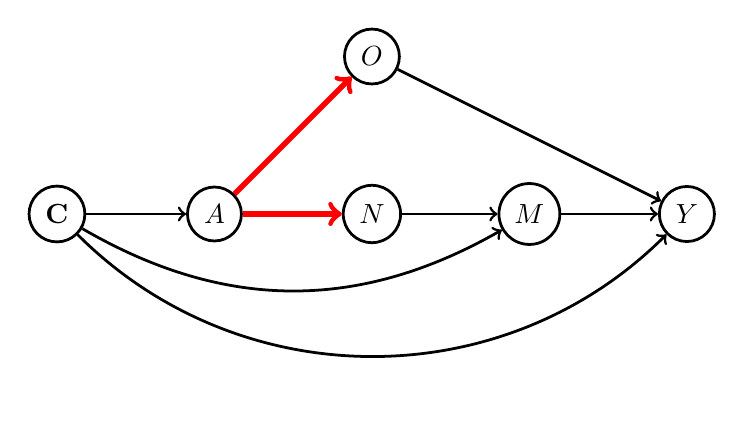
\begin{tikzpicture}[baseline={(A)}, 
    %.8, 
    ->, line width=1pt]
    \tikzstyle{every state}=[draw=none]
    \node[shape=circle, draw] (C) at (-2,0) {${\bf C}$};
    \node[shape=circle, draw] (A) at (0,0) {$A$};
    \node[shape=circle, draw] (N) at (2,0) {$N$};
    \node[shape=circle, draw] (O) at (2,2) {$O$};
    \node[shape=circle, draw] (M) at (4,0) {$M$};
    \node[shape=circle, draw] (Y) at (6,0) {$Y$};
    
    
      \path     (C) edge (A)
                (C) edge  [bend right=30] (M)
                (C) edge  [bend right=45] (Y)
                (M) edge (Y)
                (A) edge  [color=red, line width=2pt] (N)
                (A) edge  [color=red, line width=2pt] (O)
                (N) edge (M)
                (O) edge (Y)
                          ;
    \end{tikzpicture}
    \caption{The extended mediation DAG with separable effects of $A$ on $M$ and $Y$.\label{fig:DAG3}}
\end{figure}
The model asserts that the effect of $A$ on $M$ and $Y$ can be separated into two components, $N$ and $O$, where $N$ completely mediates the effect of $A$ on $M$ and has no direct effect on $Y$, and $O$ completely mediates the direct effect of $A$ on $Y$ and has no effect on $M$. \cite{robins2010alternative} showed that the NIE is nonparametrically identified under the FFRCISTG corresponding to a version of the DAG in Figure \ref{fig:DAG3} where $A$ is randomized, such that there is no arrow from $\bf C$ to $A$. The extension to the observational setting is trivial.
\begin{theorem}
    \label{thm:separable-effects}
    Under the FFRCISTG corresponding to the DAG in Figure \ref{fig:DAG3}, the NIE$^{\text{R}}$ is equal to the NIE and satisfies the indirect effect measure criteria.
\end{theorem}

Another way the sharp null and sharper null criteria can be recovered is if %$Y(a,m)\neq Y(a,m')$ almost surely for all $m$ and $m'$ in the support of $M$, i.e., if 
$M$ affects $Y$ for every individual. 
\begin{theorem}
    \label{thm:m-always-affects-y}
    Suppose that for each subject $i$, either $Y_i(a^*,m)\neq Y_i(a^*,m')$ or $Y_i(a,m)\neq Y_i(a,m')$ for all $m$ and $m'$ in the support of $M$. Then under the FFRCISTG corresponding to the DAG in Figure 1, the NIE$^{\text{R}}$ satisfies both the sharp null and sharper null criteria.
\end{theorem}
In this case, the NIE is not nonparametrically identified, so the NIE$^{\text{R}}$ does hold an advantage over the NIE as an indirect effect measure in this setting. However, it seems unlikely in most practical applications that one would have knowledge that there is an effect of $M$ on $Y$ for each individual. Additionally, it is not clear in this case whether the NIE$^{\text{R}}$ satisfies the monotonicity criterion.

\section{Proofs}
\begin{proof}[Proof of Theorem 1]
%    The proof follows from the following counterexample. 
%For a true indirect effect to exist, there must be an individual indirect effect for at least one subject, i.e., for one or more subjects, their exposure must affect their intermediate variable, and their intermediate variable must affect their outcome. Thus, for a true causal contrast to have an in direct effect interpretation, it should take its null value (e.g., zero on the difference scale) whenever there is no individual-level indirect effect for any subject. However, as the following counterexample demonstrates, NIE$^{\mathrm{R}}$ can be nonzero even when no individual-level indirect effect exists for any subject.
Suppose $A$ is randomized such that ${\bf C}$ is the empty set with $a=1$ and $a^*=0$, 
and suppose the counterfactual distribution belonging to the NPSEM-IE is
\begin{align*}
    A &= \varepsilon_A \\
    L &= A\varepsilon_L + (1-A)(1-\varepsilon_L) \\
    M &= (A+L-AL)\varepsilon_M + (1-A)(1-L)(1-\varepsilon_M) \\
    Y &= (1-A)LM+A(L+M-LM),
\end{align*}
where $\varepsilon_A\sim \text{Bernoulli}(1/2)$, $\varepsilon_L\sim \text{Bernoulli}(\pi)$, $\varepsilon_M\sim \text{Bernoulli}(\beta)$, and $\varepsilon_A$, $\varepsilon_L$, and $\varepsilon_M$ are mutually independent. Thus, when $\varepsilon_L = 0$, 
\[M(a^*)=M\{a^*,L(a^*)\}=M(a^*,1)=\varepsilon_M=M(a,0)=M\{a,L(a)\}=M(a),\] 
so $A$ does not affect $M$, and $Y\{a',M(a)\} = Y\{a',M(a^*)\}$ for both $a'\in\{a^*,a\}$. When $\varepsilon_L = 1$,
\begin{align*}
    Y(a,1) &= Y\{a,L(a),1\} = f_Y(a,a,1) = 1 = f_Y(a,a,0) = Y\{a,L(a),0\} = Y(a,0)
\end{align*}
and
\begin{align*}
    Y(a^*,1) &= Y\{a^*,L(a^*),1\} = f_Y(a^*,a^*,1) = 0\\ 
    &= f_Y(a^*,a^*,0) = Y\{a^*,L(a^*),0\} = Y(a^*,0),
\end{align*}
\begin{comment}
\begin{align*}
    Y\{a,M(a)\}&=f_Y[a,L(a),M\{a,L(a)\}]=f_Y(a,a,\varepsilon_M)=1\\
    &=f_Y(a,a,1-\varepsilon_M)=f_Y[a,L(a),M\{a^*,L(a^*)\}]=Y\{a,M(a^*)\},
\end{align*}
and
\begin{align*}
    Y\{a^*,M(a)\}&=f_Y[a^*,L(a^*),M\{a,L(a)\}]=f_Y(a^*,a^*,\varepsilon_M)=0\\
    &=f_Y(a^*,a^*,1-\varepsilon_M)=f_Y[a^*,L(a^*),M\{a^*,L(a^*)\}]=Y\{a^*,M(a^*)\},
\end{align*}
\end{comment}
so $M$ does not affect $Y$. Thus, the sharper mediational null holds %there can be no individual-level indirect effect 
since $\varepsilon_L$ is either zero or one. However, under this counterfactual distribution, we have $\mathrm{NIE}^{\mathrm{R}}=\pi(1-\pi)(2\beta-1)$, 
%$\pi\{2(1-2\beta)\pi+2\beta-1\}$, 
which does not equal zero in general. In fact, NIE$^{\mathrm{R}}$ goes to -1/4 as $\pi$ goes to 1/2 and $\beta$ goes to 0, and NIE$^{\mathrm{R}}$ goes to 1/4 as $\pi$ goes to 1/2 and $\beta$ goes to 1, hence NIE$^{\mathrm{R}}$ is not bounded away from -1/4 or 1/4 even when there is no individual-level indirect effect for any subject. Thus, the NIE$^{\mathrm{R}}$ does not satisfy the sharper null criterion, and therefore neither does it satisfy the sharp null or monotonicity criteria.
\end{proof}

\begin{proof}[Proof of Theorem 2]
    The sharp mediational null implies that $Y_{k}\{a,M(a^*)\} = Y_{k}\{a,M(a)\}$ for all $k$, hence either $M_i(a) = M_i(a^*)$ for all $i$ or $Y_j(a,m) = Y_j(a,m')$ for all $j$ and $m\neq m'$. In the first case, we have $f_{M(a)}(m)=f_{M(a^*)}(m)$ for all $m$, which implies $f_{M\mid A, {\bf C}}(m\mid a, {\bf C})=f_{M\mid A, {\bf C}}(m\mid a^*, {\bf C})$ almost surely for all $m$, so %$\text{NIE}^{\text{R}} = \Psi_L^{\text{NIE}^{\text{R}}}(P)=0$. 
    \begin{align*}
        \text{NIE}^{\text{R}} =&\; E\bigg[\int_m \int_{\boldsymbol{\ell}} E(Y\mid m,\boldsymbol{\ell},a,{\bf C})dF_{{\bf L}\mid A, {\bf C}}(\boldsymbol{\ell}\mid a, {\bf C})\\
        &\times \{dF_{M\mid A,{\bf C}}(m\mid a,{\bf C}) - dF_{M\mid A,{\bf C}}(m\mid a^*,{\bf C})\}\bigg]\\
        =&\; 0.
    \end{align*}
    In the second case, $f_{Y(a,m)}(y) = f_{Y(a,m')}(y)$ for all $m$, which implies $E(Y\mid m,{\bf L},a,{\bf C}) = E(Y\mid {\bf L},a,{\bf C})$ almost surely for all $m$, so
    \begin{align*}
        \text{NIE}^{\text{R}} =&\; E\bigg[\int_m \int_{\boldsymbol{\ell}} E(Y\mid m,\boldsymbol{\ell},a,{\bf C})dF_{{\bf L}\mid A, {\bf C}}(\boldsymbol{\ell}\mid a, {\bf C})\\
        &\times \{dF_{M\mid A,{\bf C}}(m\mid a,{\bf C}) - dF_{M\mid A,{\bf C}}(m\mid a^*,{\bf C})\}\bigg]\\
        =&\; E\bigg[\int_{\boldsymbol{\ell}} E(Y\mid \boldsymbol{\ell},a,{\bf C})dF_{{\bf L}\mid A, {\bf C}}(\boldsymbol{\ell}\mid a, {\bf C})\\
        &\times \int_m \{dF_{M\mid A,{\bf C}}(m\mid a,{\bf C}) - dF_{M\mid A,{\bf C}}(m\mid a^*,{\bf C})\}\bigg]\\
        =&\; 0.
    \end{align*}
    Thus, in either case, $\text{NIE}^{\text{R}}=0$, so the $\text{NIE}^{\text{R}}$ satisfies the sharp null criterion, and in turn the sharper null criterion.

    Now consider the following counterfactual distribution belonging to the NPSEM-IE corresponding to the DAG in Figure 2:
    \begin{align*}
        A &= \varepsilon_A \\
        L &= (1-A)I(\varepsilon_L = 0) + AI(\varepsilon_L = 1) + 2I(\varepsilon_L = 2) \\
        M &= \{(A+L-AL)\varepsilon_M + (1-A)(1-L)(1-\varepsilon_M)\}I(L \neq 2) + AI(L = 2) \\
        Y &= \{(1-A)LM+A(L+M-LM)\}I(L \neq 2) + MI(L = 2),
    \end{align*}
    where $\varepsilon_A\sim \text{Bernoulli}(1/2)$, $\varepsilon_L\sim \text{Categorical}(\pi_0,\pi_1,\pi_2)$, $\varepsilon_M\sim \text{Bernoulli}(\beta)$, and $\varepsilon_A$, $\varepsilon_L$, and $\varepsilon_M$ are mutually independent. When $\varepsilon_L\neq 2$, this reduces to the distribution in the proof of Theorem 1, so $Y\{a',M(a^*)\}=Y\{a',M(a)\}$ for each $a'\in\{a^*,a\}$. When $\varepsilon_L=2$, $L(a')=2$, $M(a')=a'$, and $Y(a',m)=Y(a',2,m)=m$ for all $a'\in\{a^*,a\}$ and $m$, so 
    \[Y\{a,M(a)\}=Y(a,2,a)=a > a^* = Y(a,2,a^*) = Y\{a,M(a^*)\},\] 
    and 
    \[Y\{a^*,M(a)\} = Y(a^*,2,a) = a > a^* = Y(a^*,2,a^*) = Y\{a^*,M(a^*)\}.\]
    Thus, mediational monotonicity holds. However, $\text{NIE}^{\text{R}}=\pi_1(1-\pi_1)(2\beta-1)+\pi_2$, which goes to $\pi_2-1/4$ as $\pi_1\rightarrow 1/2$ and $\beta\rightarrow 0$. Thus, when $\pi_2<1/4$, the $\text{NIE}^{\text{R}}$ can be negative, which violates the monotonicity criterion.
\end{proof}

\begin{proof}[Proof of Theorem 3]
    Consider the following counterfactual distribution. Suppose $A\sim \text{Bernoulli}(1/2)$, i.e., $A$ is randomized, $M(a)\sim\text{Bernoulli}(\pi)$, and 
    \begin{align*}
        \{Y(a,0), Y(a,1)\} &= \left\{\begin{array}{ll}
            (0, 0) & \text{with probability } \beta_1 \\
            (0, 1) & \text{with probability } \beta_2 \\
            (1, 0) & \text{with probability } \beta_3 \\
            (1, 1) & \text{with probability } \beta_4 \\
        \end{array}\right.,
    \end{align*}
    which are independent of $M(a)$, where $\beta_1+\beta_2+\beta_3+\beta_4=1$. Suppose further that 
    \[M(a^*)=Y(a,0)Y(a,1) + M(a)\lvert Y(a,1)-Y(a,0)\rvert,\] 
    and
    \begin{align*}
        \{Y(a^*,0), Y(a^*,1)\} &= \left\{\begin{array}{ll}
            (0, 0) & \text{with probability } 1-\gamma \\
            (1, 1) & \text{with probability } \gamma \\
        \end{array}\right.,
    \end{align*}
    where $0<\gamma<1$. This counterfactual distribution belongs to the FFRCISTG model, but not the NPSEM-IE since $M(a^*)$ is independent of neither $Y(a,0)$ nor $Y(a,1)$. 
    
    We have $Y(a^*,0) = Y(a^*,1)$ almost surely, and when $Y(a,0)\neq Y(a,1)$, $M(a^*)=M(a)$. 
\begin{comment}    
    When $M(a)=0$, we have %$Y\{a,M(a^*)\} = Y(a,0)I\{\} $
    \begin{align*}
        Y\{a,M(a^*)\} &= Y(a,0)\{1-M(a^*)\} + Y(a,1)M(a^*)\\
        &= Y(a,0)\{1-Y(a,0)Y(a,1)\} + Y(a,0)Y(a,1)^2\\
        &= Y(a,0) - Y(a,0)Y(a,1) + Y(a,0)Y(a,1)\\
        &= Y\{a,M(a)\}.
    \end{align*}

    When $M(a)=1$, we have
    \begin{align*}
        Y\{a,M(a^*)\} =& Y(a,0)\{1-M(a^*)\} + Y(a,1)M(a^*)\\
        =& Y(a,0)\{1-Y(a,0)Y(a,1)-\lvert Y(a,1)-Y(a,0)\rvert\}\\ 
        &+ Y(a,1)\{Y(a,0)Y(a,1) + \lvert Y(a,1)-Y(a,0)\rvert\}\\
        =& Y(a,0) - Y(a,0)Y(a,1) + Y(a,0)Y(a,1)\\ 
        &+ \{Y(a,1)-Y(a,0)\}\{Y(a,0) + Y(a,1) - 2Y(a,0)Y(a,1)\}\\
        =& Y(a,0) + Y(a,0)Y(a,1) + Y(a,1) - 2Y(a,0)Y(a,1)\\ 
        &- Y(a,0) - Y(a,0)Y(a,1) + 2Y(a,0)Y(a,1)\\
        =& Y\{a,M(a)\}.
    \end{align*}
\end{comment}
    Thus, the sharper mediational null holds. However, under this counterfactual distribution, we have %$\text{NIE}^{\text{R}} = \beta_4(\beta_3 - \beta_2) + \pi\{\beta_2(1-\beta_2)-\beta_3(1-\beta_3)\}$
    $\text{NIE}^{\text{R}} = \{(1-\pi)\beta_4 - \pi\beta_1\}(\beta_3 - \beta_2)$, which does not equal zero in general. This will go to $1/4$ as $\pi\rightarrow 0$, $\beta_1\rightarrow 0$, $\beta_2\rightarrow 0$, $\beta_3\rightarrow 1/2$, and $\beta_4\rightarrow 1/2$, and will go to $-1/4$ as $\pi\rightarrow 0$, $\beta_1\rightarrow 0$, $\beta_2\rightarrow 1/2$, $\beta_3\rightarrow 0$, and $\beta_4\rightarrow 1/2$. Thus, the $\text{NIE}^{\text{R}}$ fails to satisfy the sharper null criterion, and in turn the sharp null criterion as well.
\end{proof}

\begin{proof}[Proof of Theorem 4]
    %First observe that $E\{Y(a,m)\mid C=c\} = E(Y\mid A=a, M=m, C=c)$ for all $m$ implies that $E[Y\{a,M(a^*)\}\mid C=c] = E\{Y\mid A=a, M=M(a^*), C=c\}$.
    Under this model, $E[Y\{a,M(a)\}]$ is known to be identified by $E\{E(Y\mid a,{\bf C})\}$, which equals $E[E\{E(Y\mid M,a,{\bf C})\mid a,{\bf C}\}]$. Observe that no mean interaction given $M(a^*)$ and $\bf C$
    \[E\{Y(a',m')-Y(a',m'')-Y(a'',m')+Y(a'',m'')\mid M(a^*),{\bf C}\}=0\]
    implies the weaker no mean interaction statement given $\bf C$ alone:
    \[E\{Y(a',m')-Y(a',m'')-Y(a'',m')+Y(a'',m'')\mid {\bf C}\}=0.\]
    For a given fixed level $m'$,
    \begin{align*}
        &E\left[Y\left\{a,M(a^*)\right\}\right]\\ 
        =&E\left[\int_m E\left\{Y\left(a,m\right)\mid M(a^*)=m, {\bf C}\right\}dF_{M(a^*)\mid{\bf C}}(m\mid {\bf C})\right]\\ 
        =&E\left[\int_m E\left\{Y(a,m')+Y(a^*,m)-Y(a^*,m')\mid M(a^*)=m, {\bf C}\right\}dF_{M(a^*)\mid{\bf C}}(m\mid {\bf C})\right]\\ 
        =&E\left(E\left[E\left\{Y(a,m')\mid M(a^*), {\bf C}\right\}\mid {\bf C}\right]\right.\\
        &+\int_m E\left\{Y(a^*,m)\mid M(a^*)=m, {\bf C}\right\}dF_{M(a^*)\mid{\bf C}}(m\mid {\bf C})\\
        &\left.-E\left[E\left\{Y(a^*,m')\mid M(a^*), {\bf C}\right\}\mid {\bf C}\right]\right)\\ 
        =&E\left[E\left\{Y(a,m')\mid {\bf C}\right\}+\int_m E\left\{Y(a^*,m)\mid {\bf C}\right\}dF_{M(a^*)\mid{\bf C}}(m\mid {\bf C})-E\left\{Y(a^*,m')\mid {\bf C}\right\}\right]\\ 
        %=& E\left(E\left[Y\left\{a,M(a^*)\right\}\mid C\right]\right)\\
        %=& E\left[Y(a, m') + Y\left\{a^*, M(a^*)\right\} - Y(a^*, m')\right]\\
        %=& E\left(E\left[Y(a, m') + Y\left\{a^*, M(a^*)\right\} - Y(a^*, m')\mid {\bf C}\right]\right)\\
        %=& E\left[\int_m E\left\{Y(a, m') + Y(a^*, m) - Y(a^*, m')\mid M(a^*), C\right\}dF_{M(a^*)\mid C}(m\mid C)d\mu(m)\right]\\
        %=& E\left[E\left\{Y\mid A=a, M=M(a^*), C\right\}\right]\\
        %=& E\left(E\left\{Y(a, m')\mid C\right\} + E\left[Y\left\{a^*, M(a^*)\right\}\mid C\right] - E\left\{Y(a^*, m')\mid C\right\}\right)\\
        %=& E\left(E\left\{Y(a, m')\mid C\right\} + \int_m E\left[Y\left\{a^*, M(a^*)\right\}\mid M(a^*)=m, C\right]dF_{M(a^*)\mid C}(m\mid C)\right.\\ 
        %&- \left.E\left\{Y(a^*, m')\mid C\right\}\right)\\
        %=& E\left[E\left\{Y(a, m')\mid {\bf C}\right\} + \int_m E\left\{Y\left(a^*, m\right)\mid M(a^*)=m, {\bf C}\right\}dF_{M(a^*)\mid {\bf C}}(m\mid {\bf C})\right.\\ 
        %&- \left.E\left\{Y(a^*, m')\mid {\bf C}\right\}\right]\\
        =& E\left[\int_m E\left\{Y(a, m')+Y\left(a^*, m\right)-Y(a^*, m')\mid {\bf C}\right\}dF_{M(a^*)\mid {\bf C}}(m\mid {\bf C})\right]\\
        =& E\left[\int_m E\left\{Y(a, m)\mid {\bf C}\right\}dF_{M(a^*)\mid {\bf C}}(m\mid {\bf C})\right]\\
        =& E\left\{\int_m E\left(Y\mid M=m, A=a, {\bf C}\right)dF_{M\mid A,{\bf C}}(m\mid a^*, {\bf C})\right\}\\
        =& E\left[E\left\{E\left(Y\mid M, A=a, {\bf C}\right)\mid A=a^*, {\bf C}\right\}\right].
    \end{align*}
    Thus, $\text{NIE}=\Psi^{\text{NIE}}(P)$.

    Under the FFRCISTG corresponding to the DAG in Figure 1, the NIE$^{\text{R}}$ is also known to be identified by $=\Psi^{\text{NIE}}(P)$. By marginalizing over the four-way decomposition in \cite{vanderweele2014unification}, $\text{TE} = \text{CDE}(m) + \text{INT}_{\text{ref}}(m,m') + \text{NIE}$, where 
    \[\text{INT}_{\text{ref}}(m,m') = E[\{Y(a,m)-Y(a,m')-Y(a^*,m)+Y(a^*,m')\}M(a^*)]\]
    for all $m$ and $m'$. Under the no mean causal interaction assumption, we have
    \begin{align*}
        \text{INT}_{\text{ref}}(m,m') &= E[\{Y(a,m)-Y(a,m')-Y(a^*,m)+Y(a^*,m')\}M(a^*)] \\
        &= E[E\{Y(a,m)-Y(a,m')-Y(a^*,m)+Y(a^*,m')\mid M(a^*),{\bf C}\}M(a^*)] \\
        &= 0.
    \end{align*}
    Thus, $\text{NIE} = \text{TE} - \text{CDE}(m) = \text{PE}(m)$.
\end{proof}

\begin{proof}[Proof of Corollary 1]
    Since the NIE$^{\text{R}}$ and $\text{PE}(m)$ are also identified by $\Psi^{\text{NIE}}(P)$ and the NIE satisfies the sharp null criterion, the NIE$^{\text{R}}$ and $\text{PE}(m)$ must also satisfy the indirect effect criteria in this setting.
\end{proof}

\begin{proof}[Proof of Theorem 5]
    First, we have
    \begin{align*}
        &E\left[Y\left\{a,M(a)\right\}\right]\\ 
        %=&\; E\left[Y\left\{a,{\bf L}(a),M(a)\right\}\right]\\ 
        =&\; E\left[\int_{\boldsymbol{\ell}} \int_m E\left\{Y\left(a,\boldsymbol{\ell},m\right)\mid M(a)=m, {\bf L}(a)=\boldsymbol{\ell}, {\bf C}\right\}dF_{M(a)\mid {\bf L}(a), {\bf C}}(m\mid \boldsymbol{\ell}, {\bf C})dF_{{\bf L}(a)\mid {\bf C}}(\boldsymbol{\ell}\mid {\bf C})\right]\\ 
        =&\;  E\left[\int_{\boldsymbol{\ell}} \int_m E\left\{Y(a, \boldsymbol{\ell}, m)\mid {\bf C}\right\}dF_{M(a)\mid {\bf C}}(m\mid {\bf C})dF_{{\bf L}(a)\mid {\bf C}}(\boldsymbol{\ell}\mid {\bf C})\right]\\
        =&\;  E\left\{\int_{\boldsymbol{\ell}} \int_m E\left(Y\mid m, \boldsymbol{\ell}, a, {\bf C}\right)dF_{M\mid A,{\bf C}}(m\mid a, {\bf C})dF_{{\bf L}\mid A, {\bf C}}(\boldsymbol{\ell}\mid a,{\bf C})\right\}.
    \end{align*}

    %(???) Under this model, $E[Y\{a,M(a)\}]$ is known to be identified by %$E\{E(Y\mid a,{\bf C})\}$, which equals 
    %\[E\left[\int_m E\left\{E(Y\mid m, {\bf L}, a, {\bf C}) \mid a, {\bf C}\right\}dF_{M\mid A,{\bf C}}(m\mid a, {\bf C})\right].\]
    From the proof of Theorem 4, the derivation showing
    \[E\left[Y\left\{a,M(a^*)\right\}\right] = E\left[\int_m E\left\{Y(a, m)\mid {\bf C}\right\}dF_{M(a^*)\mid {\bf C}}(m\mid {\bf C})\right]\]
    follows identically under the FFRCISTG corresponding to the DAG in Figure 2; however, $E\left\{Y(a, m)\mid {\bf C}\right\}$ is identified differently due to the presence of $\bf L$. Instead, we have
    \begin{align*}
        &E\left[\int_m E\left\{Y(a, m)\mid {\bf C}\right\}dF_{M(a^*)\mid {\bf C}}(m\mid {\bf C})\right]\\
        =&\; E\left\{\int_m\int_{\boldsymbol{\ell}} E\left(Y\mid m, \boldsymbol{\ell}, a, {\bf C}\right)dF_{{\bf L}\mid A, {\bf C}}(\boldsymbol{\ell}\mid a, {\bf C})dF_{M\mid A, {\bf C}}(m\mid a^*, {\bf C})\right\}.
    \end{align*}
    Thus, $\text{NIE}=\Psi^{\text{NIE}_{L}^{\text{R}}}(P)$.
\end{proof}

\begin{proof}[Proof of Corollary 2]
    Since the NIE$^{\text{R}}$ is also identified by $\Psi^{\text{NIE}_L^{\text{R}}}(P)$ and the NIE satisfies the sharp null criterion, the NIE$^{\text{R}}$ must also satisfy the sharp null criterion in this setting, which in turn implies the NIE$^{\text{R}}$ satisfies the sharper null criterion.
\end{proof}

\begin{proof}[Proof of Theorem \ref{thm:NIE-RL}]
    For each $a'\in\{a^*,a\}$,
    \begin{align*}
        &E\left[Y\left\{a,G(a'\mid {\bf C}, {\bf L})\right\}\right]\\ 
        &= E\left[\int_{\boldsymbol\ell}\int_mE\left\{Y(a,m)\mid G(a'\mid {\boldsymbol\ell},{\bf C})=m,{\boldsymbol\ell},{\bf C}\right\}dF_{G(a'\mid {\bf L}, {\bf C})\mid {\bf L}, {\bf C}}(m\mid {\boldsymbol\ell}, {\bf C})dF_{\bf L\mid C}(\boldsymbol\ell\mid {\bf C})\right]\\
        &= E\left[\int_{\boldsymbol\ell}\int_mE\left\{Y(a,m)\mid {\boldsymbol\ell},{\bf C}\right\}dF_{M(a')\mid {\bf L}, {\bf C}}(m\mid {\boldsymbol\ell}, {\bf C})dF_{\bf L\mid C}(\boldsymbol\ell\mid {\bf C})\right]\\
        &= E\left[\int_{\boldsymbol\ell}\int_mE\left\{Y(a,m)\mid m,{\boldsymbol\ell},a,{\bf C}\right\}dF_{M(a')\mid {\bf L}, A, {\bf C}}(m\mid {\boldsymbol\ell}, a', {\bf C})dF_{\bf L\mid C}(\boldsymbol\ell\mid {\bf C})\right]\\
        &= E\left\{\int_{\boldsymbol\ell}\int_mE\left(Y\mid m,{\boldsymbol\ell},a,{\bf C}\right)dF_{M\mid {\bf L}, A, {\bf C}}(m\mid {\boldsymbol\ell}, a', {\bf C})dF_{\bf L\mid C}(\boldsymbol\ell\mid {\bf C})\right\},
    \end{align*}
    hence
    \begin{align*}
        &E\left[Y\left\{a,G(a\mid {\bf C}, {\bf L})\right\}\right]-E\left[Y\left\{a,G(a^*\mid {\bf C}, {\bf L})\right\}\right]\\
        &= E\left[\int_{\boldsymbol\ell}\int_mE\left(Y\mid m,{\boldsymbol\ell},a,{\bf C}\right)\left\{dF_{M\mid {\bf L}, A, {\bf C}}(m\mid {\boldsymbol\ell}, a, {\bf C})\right.\right.\\
        &\left.\left.-dF_{M\mid {\bf L}, A, {\bf C}}(m\mid {\boldsymbol\ell}, a^*, {\bf C})\right\}dF_{\bf L\mid C}(\boldsymbol\ell\mid {\bf C})\right].
    \end{align*}
    Under the counterfactual distribution in the proof of Theorem 1,
    \[E\left[Y\left\{a,G(a\mid {\bf C}, {\bf L})\right\}\right]-E\left[Y\left\{a,G(a^*\mid {\bf C}, {\bf L})\right\}\right] = \beta - 1/2.\]
    Thus, while the sharp mediational null holds under this counterfactual distribution, this effect measure is not zero in general, and may take any value in $(-1/2,1/2)$ depending on the value of $\beta$.
\end{proof}

\begin{proof}[Proof of Theorem \ref{thm:NIE-RLa}]
    \begin{align*}
        &E\left(Y\left[a,G\left\{a\mid {\bf C}, {\bf L}(a)\right\}\right]\right)\\
        =& E\left(\iint\limits_{{\boldsymbol \ell},m}E\left[Y(a,m)\mid G\{a\mid C,{\bf L}(a)\}=m,{\bf L}(a)={\boldsymbol \ell}, C\right]\right.\\
        &\times \left.dF_{G\{a\mid C,{\bf L}(a)\}\mid {\bf L}(a),C}(m\mid {\boldsymbol \ell},C)dF_{{\bf L}(a)\mid C}({\boldsymbol \ell}\mid C)\right)\\
        =& E\left[\iint\limits_{{\boldsymbol \ell},m}E\left\{Y(a,{\boldsymbol \ell},m)\mid {\bf L}(a)={\boldsymbol \ell}, C\right\}dF_{M(a)\mid {\bf L}(a),C}(m\mid {\boldsymbol \ell},C)dF_{{\bf L}(a)\mid C}({\boldsymbol \ell}\mid C)\right]\\
        =& E\left[\iint\limits_{{\boldsymbol \ell},m}E\left\{Y(a,{\boldsymbol \ell},m)\mid M(a,{\boldsymbol \ell})=m, {\bf L}(a)={\boldsymbol \ell}, C\right\}dF_{M(a,{\boldsymbol \ell}), {\bf L}(a)\mid C}(m, {\boldsymbol \ell}\mid C)\right]\\
        =& E\left[Y\{a,M(a)\}\right],
    \end{align*}
    and
    \begin{align*}
        &E\left(Y\left[a,G\left\{a^*\mid {\bf C}, {\bf L}(a^*)\right\}\right]\right)\\
        =& E\left(\iiint\limits_{{\boldsymbol \ell^*},{\boldsymbol \ell},m}E\left[Y(a,m)\mid G\{a^*\mid C,{\bf L}(a^*)\}=m,{\bf L}(a^*)={\boldsymbol \ell^*}, {\bf L}(a)={\boldsymbol \ell}, C\right]\right.\\
        &\times \left.dF_{G\{a^*\mid C,{\bf L}(a^*)\}\mid {\bf L}(a^*),{\bf L}(a),C}(m\mid {\boldsymbol \ell^*},{\boldsymbol \ell},C)dF_{{\bf L}(a^*),{\bf L}(a)\mid C}({\boldsymbol \ell^*},{\boldsymbol \ell}\mid C)\right)\\
        =& E\left[\iiint\limits_{{\boldsymbol \ell^*},{\boldsymbol \ell},m}E\left\{Y(a,{\boldsymbol \ell},m)\mid M(a^*,{\boldsymbol \ell^*})=m,{\bf L}(a^*)={\boldsymbol \ell^*}, {\bf L}(a)={\boldsymbol \ell}, C\right\}\right.\\
        &\times \left.dF_{G\{a^*\mid C,{\bf L}(a^*)\}\mid {\bf L}(a^*),C}(m\mid {\boldsymbol \ell^*},C)dF_{{\bf L}(a^*),{\bf L}(a)\mid C}({\boldsymbol \ell^*},{\boldsymbol \ell}\mid C)\right]\\
        =& E\left(\iiint\limits_{{\boldsymbol \ell^*},{\boldsymbol \ell},m}E\left[Y\{a,M(a^*)\}\mid M(a^*,{\boldsymbol \ell^*})=m,{\bf L}(a^*)={\boldsymbol \ell^*}, {\bf L}(a)={\boldsymbol \ell}, C\right]\right.\\
        &\times \left.dF_{M(a^*)\mid {\bf L}(a^*),C}(m\mid {\boldsymbol \ell^*},C)dF_{{\bf L}(a^*),{\bf L}(a)\mid C}({\boldsymbol \ell^*},{\boldsymbol \ell}\mid C)\right)\\
        =& E\left(\iiint\limits_{{\boldsymbol \ell^*},{\boldsymbol \ell},m}E\left[Y\{a,M(a^*)\}\mid M(a^*,{\boldsymbol \ell^*})=m,{\bf L}(a^*)={\boldsymbol \ell^*}, {\bf L}(a)={\boldsymbol \ell}, C\right]\right.\\
        &\times \left.dF_{M(a^*), {\bf L}(a^*),{\bf L}(a),C}(m,{\boldsymbol \ell^*},{\boldsymbol \ell},C)\right)\\
        =& E\left[Y\left\{a,M(a^*)\right\}\right],
    \end{align*}
    hence
    \[E\left(Y\left[a,G\left\{a\mid {\bf C}, {\bf L}(a)\right\}\right]\right)-E\left(Y\left[a,G\left\{a^*\mid {\bf C}, {\bf L}(a^*)\right\}\right]\right)=\text{NIE}.\]
    Since the NIE is not nonparametrically identified in this setting, neither then is \[E\left(Y\left[a,G\left\{a\mid {\bf C}, {\bf L}(a)\right\}\right]\right)-E\left(Y\left[a,G\left\{a^*\mid {\bf C}, {\bf L}(a^*)\right\}\right]\right).\]
\end{proof}

\begin{proof}[Proof of Theorem \ref{thm:no-LM-interaction}]
    We can infer from \cite{tchetgen2014identification} that under the assumption of no mean ${\bf L}$--$M$ interaction on $Y$ on the additive scale, the NIE is nonparametrically identified by
    \[E\left[\int_m E(Y\mid m,{\boldsymbol \ell'},a,C)\left\{dF_{M\mid A,C}(m\mid a,C)-dF_{M\mid A,C}(m\mid a^*,C)\right\}\right]\]
    for any ${\boldsymbol \ell'}$. Under this assumption, we also have
    \begin{align*}
        \text{NIE}^{\text{R}} =& E\left[\int_m E\left\{E(Y\mid m,{\bf L},a,{\bf C})\mid a,{\bf C}\right\}\{dF_{M\mid A,{\bf C}}(m\mid a,{\bf C}) - dF_{M\mid A,{\bf C}}(m\mid a^*,{\bf C})\}\right]\\
        =& E\left[\int_m E\left\{E(Y\mid m',{\bf L},a,{\bf C}) + E(Y\mid m,{\boldsymbol \ell'},a,{\bf C}) - E(Y\mid m',{\boldsymbol \ell'},a,{\bf C})\mid a,{\bf C}\right\}\right.\\
        &\times\left.\{dF_{M\mid A,{\bf C}}(m\mid a,{\bf C}) - dF_{M\mid A,{\bf C}}(m\mid a^*,{\bf C})\}\right]\\
        =& E\left[\int_m E(Y\mid m,{\boldsymbol \ell'},a,C)\left\{dF_{M\mid A,C}(m\mid a,C)-dF_{M\mid A,C}(m\mid a^*,C)\right\}\right]\\
        =& \text{NIE}
    \end{align*}
    for all ${\boldsymbol \ell'}$.
\end{proof}

\begin{proof}[Proof of Theorem \ref{thm:separable-effects}]
    The FFRCISTG corresponding to the DAG in Figure 3 is a submodel of the FFRCISTG corresponding to the DAG in Figure 1, hence the NIE$^{\text{R}}$ is nonparametrically identified by $\Psi^{\text{NIE}}(P)$ as it is in the larger model. Since the NIE is also nonparametrically identified by $\Psi^{\text{NIE}}(P)$ under this submodel, the two are equivalent, and since the NIE satisfies the sharp null criterion, so must the NIE$^{\text{R}}$.
\end{proof}

\begin{proof}[Proof of Theorem \ref{thm:m-always-affects-y}]
    In this case, the sharp mediational null implies that $M(a)=M(a^*)$ must hold almost surely, in which case $G(a)$ and $G(a^*)$ follow the same distribution, and $\text{NIE}^{\text{R}}=0$. Thus, the $\text{NIE}^{\text{R}}$ satisfies the sharp null criterion, and in turn must also satisfy the sharper null criterion.
\end{proof}

\bibliographystyle{apalike}
%\bibliographystyle{Chicago}

\bibliography{references}

\end{document}
%%% Local Variables:
%%% mode: latex
%%% TeX-master: t
%%% End:
